\section{Revisão rápida}
\label{sec:revisao}

\subsection{Integrais simples e o cálculo de áreas}
\label{sec:revisao-int1}
Um dos problemas fundamentais do cálculo é a determinação da \emph{área} sob
uma uma função $y = f(x)$ qualquer, quando $x$ varia em um intervalo
$a \le x \le b$. Esse problema é ilustrado na figura~\ref{fig:area}, abaixo:

\begin{figure}[H]
  \begin{center}
    \caption{Área sob funções: integral simples}
    \label{fig:area}
    \fbox{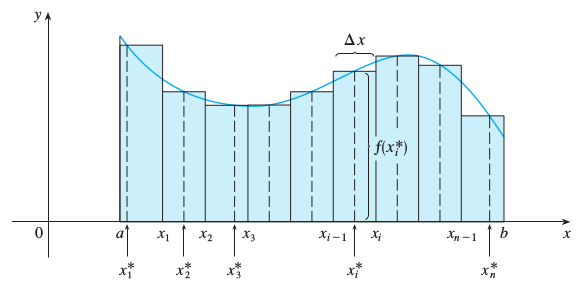
\includegraphics[scale=0.5]{imagens/int01.png}}\\
    \footnotesize{James Stewart: \emph{Cálculo} (8ª ed.,\ vol.\ 2,
      pg.\ 884)}
  \end{center}
\end{figure}

Sabemos que uma aproximação da área sob a função pode ser feita
com o seguinte procedimento:

\begin{enumerate}
  \item Dividimos o intervalo $a \le x \le b$ em $n$ intervalos
    menores iguais, $\Delta x$. Esse intervalo formará a base
    de um retângulo que será utilizado para estimar a área sob a
    função.
  \item Dentro de cada intervalo (de cada retângulo) $\Delta x$
    escolhemos um ponto de amostragem $x^*_i$ e calculamos a altura
    do retângulo, $f(x^*_i)$.
  \item A área de cada retângulo é dada então pela multiplicação de
    sua base ($\Delta x$) por sua altura ($f(x^*_i)$): área de cada
    retângulo é igual a $f(x^*_i) \Delta x$.
  \item A aproximação da área total sob a função $y = f(x)$ no
    intervalo $a \le x \le b$ é dada pela \emph{soma} das áreas de
    todos os retângulos, conforme a equação~\ref{eq:areaaprox}.
\end{enumerate}

\begin{equation}
  \label{eq:areaaprox}
  A \approx \sum_{i=1}^n f(x_i^*) \Delta x
\end{equation}
    
É fácil perceber que à medida em que dividimos o intervalo em um maior
número $n$ de retângulos (à medida em que diminuímos $\Delta x$), a
aproximação da área será melhor. No limite, quando $n$ tende ao
infinito, a área sob a curva tende ao valor exato e essa é a idéia do
cálculo integral (equação~\ref{eq:areaexata}):

\begin{equation}
  \label{eq:areaexata}
  \begin{split}
    A  &= \lim_{n \to \infty} \sum_{i=1}^n f(x_i^*) \Delta x\\
       &= \int_a^b f(x) \diff x
  \end{split}
\end{equation}


\subsection{Integrais duplas e o cálculo de volumes}
\label{sec:revisao-int2}
Uma expansão natural do problema do cálculo de áreas é o problema do
cálculo de \emph{volumes}, ou seja: dada uma função $z = f(x,y)$
qualquer, qual é o volume que está sob a função quando $x$ varia no
intervalo $a \le x \le b$ e $y$ varia no intervalo $c \le y \le d$
(ver figura~\ref{fig:volume1} abaixo):

\begin{figure}[H]
  \begin{center}
    \caption{O problema do cálculo do volume}
    \label{fig:volume1}
    \fbox{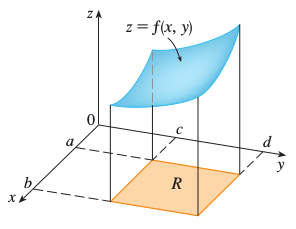
\includegraphics[scale=0.7]{imagens/int02.png}}\\
    \footnotesize{James Stewart: \emph{Cálculo} (8ª ed.,\ vol.\ 2,
      pg.\ 884)}
  \end{center}
\end{figure}

Como calcular o volume do sólido sob a função ilustrada na figura
anterior? Note que a variação no eixo $x$ e a variação no eixo $y$
delimitam uma ``base'' retangular $R$ sob a função $z = f(x,y)$. Isso
nos permite expandir o raciocínio do cálculo de áreas e obter uma
aproximação do volume com o seguinte procedimento (ver também
figura~\ref{fig:volume2} a seguir):

\begin{enumerate}
  \item Dividimos a base retangular $R$ em vários retângulos menores,
    $R_{ij}$
  \item A \emph{área de cada retângulo} $R_{ij}$ é então: $\Delta A = \Delta
    x \Delta y$    
  \item Dentro de cada retângulo $R_{ij}$ escolhemos um ponto de
    amostragem $(x^*_{ij}, y^*_{ij})$ e usamos esse ponto para
    calcular a altura do prisma, dada por: $f(x^*_{ij}, y^*_{ij})$
  \item O \emph{volume de cada prisma}, $V_{R_{ij}}$, é dado então pela multiplicação da
    área de sua base, $\Delta A$, por sua altura, $f(x^*_{ij},
    y^*_{ij})$, da seguinte maneira:
    \begin{equation}
      V_{R_{ij}} \approx f(x^*_{ij}, y^*_{ij}) \Delta A
    \end{equation}
\end{enumerate}

\begin{figure}[H]
  \begin{center}
    \caption{Dividindo o sólido sob a função em prismas}
    \label{fig:volume2}
    \fbox{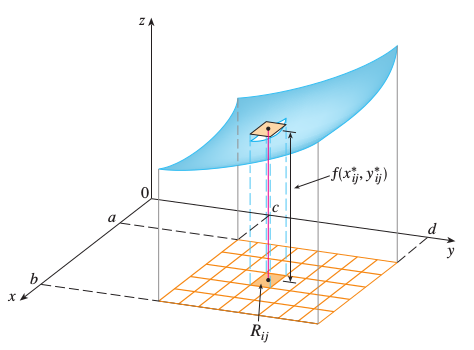
\includegraphics[scale=0.5]{imagens/int03.png}}\\
    \footnotesize{James Stewart: \emph{Cálculo} (8ª ed.,\ vol.\ 2,
      pg.\ 885)}
  \end{center}
\end{figure}

Para obter a estimativa do volume total sob a função, basta então
somar os volumes de todos os prismas (ver figura~\ref{fig:volume3}
e equação~\ref{eq:volumeaprox}):

\begin{figure}[H]
  \begin{center}
    \caption{Estimativa do volume sob a função}
    \label{fig:volume3}
    \fbox{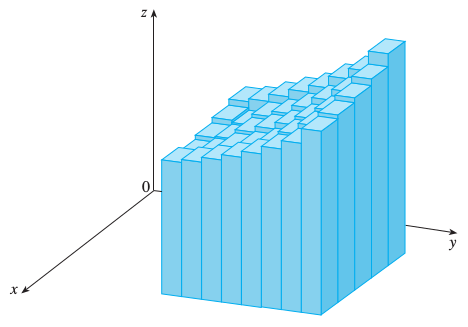
\includegraphics[scale=0.5]{imagens/int04.png}}\\
    \footnotesize{James Stewart: \emph{Cálculo} (8ª ed.,\ vol.\ 2,
      pg.\ 885)}
  \end{center}
\end{figure}

\begin{equation}
  \label{eq:volumeaprox}
  V \approx \sum_{i=1}^m \sum_{j=1}^n f(x_{ij}^*, y_{ij}^*) \Delta A
\end{equation}

Note que à medida em que dividimos o volume sob a função em um maior
número de prismas (maior número de retângulos $R_{ij}$, com intervalos
$\Delta x$ e $\Delta y$ menores e, portanto, com áreas $\Delta A$
menores), a aproximação do volume será melhor (ver
figura~\ref{fig:volume4}, a seguir):

\begin{figure}[H]
  \begin{center}
    \caption{Melhorando a estimativa do volume}
    \label{fig:volume4}
    \fbox{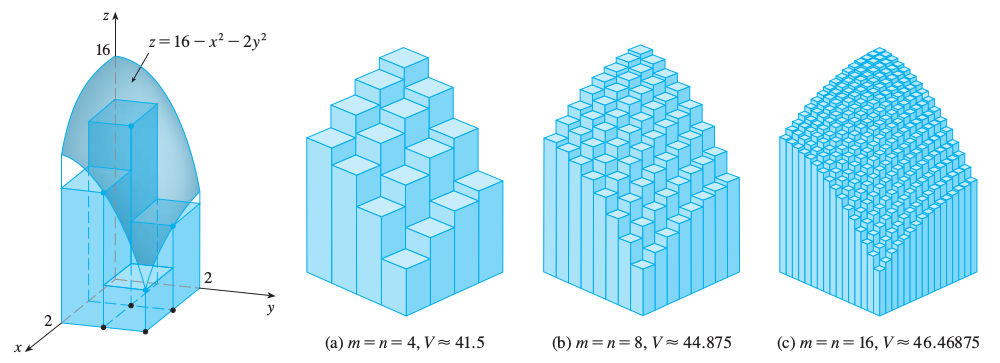
\includegraphics[scale=0.4]{imagens/int05_06.png}}\\
    \footnotesize{James Stewart: \emph{Cálculo} (8ª ed.,\ vol.\ 2,
      pg.\ 885)}
  \end{center}
\end{figure}

No limite, quanto o número de prismas tende ao infinito, o volume sob
a curva tende ao valor exato, e essa é a idéia do uso de integrais
duplas para o cálculo de volumes (equação~\ref{eq:volumeexato}):

\begin{equation}
  \label{eq:volumeexato}
  \begin{split}
      V &= \lim_{m, n \to \infty} \sum_{i=1}^m \sum_{j=1}^n f(x_{ij}^*,
      y_{ij}^*) \Delta A\\
        &= \iint\displaylimits_R f(x, y) \diff A\\
        &= \int_a^b \int_c^d f(x, y) \diff y \diff x
  \end{split}
\end{equation}
